\section{Models and Datasets}

In this section, we provide additional details for the MTL model training loop described in Section~\ref{alg:mtl_training}. 

\subsection{MTL Training} \label{appdx:training}

We use the Adam~\cite{kingma-2015-adam} and AdamW~\cite{loshchilov-2017-adamw} optimizers with weight decay to perform MTL training. Because each task could have only a small number of samples, we apply aggressive regularization to the task-specific layers to ensure that the final layers do not overfit to low-quality embeddings during training. When training our vision models where the total number of samples is small, we induce more regularization on top of weight decay by applying standard augmentations to the data such as random crops, rotations, horizontal flips, translations, and scaling. 

In our vision experiments, the CelebA dataset has very few samples per task-specific layer; 22 per celebrity after holding out samples for the weak adversary. Thus, we do two iterations of "warm start" training~\cite{nguyen-2023-flwarmup}, where we freeze the shared representation and optimize the task-specific layers for 40 epochs with with a low learning rate (e.g. $\eta = 10^{-4}$).  In our language experiments where we use BERT models, we do 20 epochs of warm start training. We also apply a linear projection on the typical, high-dimensional penultimate layer of our BERT and ResNet models to 16 or 32 dimensions in order to reduce the chance of task-specific layers overfitting. Each training step in MTL is performed over a minibatch of tasks, rather than the entire accumulated gradient of the dataset. We additionally use gradient clipping ($C = 1$), gradient normalization across tasks~\cite{chen-2018-gradnormalization}, and a smaller weight decay parameter (e.g. $\lambda = 10^{-4}$) than the task-specific layers (e.g. $\lambda = 10^{-3}$) to regularize the shared layers. In total, we train for 200-300 epochs, or communication rounds, for all of our models, passing through all of the tasks in the dataset each time.


\section{Proofs for Section~\ref{sec:mean_est}} \label{sec:proofs}

In this section, we provide the proofs for our theorems in Section~\ref{sec:mean_est}. Because the random variables in our estimation and attack are nested, we use the subscript $X$ to denote taking probability over sampling the data and subscript $\mu$ to denote taking probability over sampling tasks.
% \newtheoremstyle{plain}
\newcommand{\mubar}[0]{\bar{\mu}}
\newcommand{\muhat}[0]{\hat{\mu}}
\newcommand{\muB}[0]{\mu_B}
% \newtheoremstyle{plain}

\newtheorem*{strongadv}{Theorem~\ref{thm:strong_adv}}
\begin{strongadv}[Strong Adversary]  

Let $\tau$ be the index of the target task and suppose that the challenger sends the adversary a challenge set of $k$ samples $B$ such that, when the task is \textbf{IN}, the $k$ samples are drawn uniformly at random from $X_\tau$. Then the expected value of the statistic, $z$, when $\mu_\tau$ is \textbf{OUT} is 
    \[
        \ex{\mu, \: X}{z_{\textit{OUT}}} = 0
    \]
    and when  $\mu_\tau$ is \textbf{IN}, the expected value of $z$ is
    \[
        \ex{\mu, X}{z_{\textit{IN}}} = \frac{d}{T} \Big( \bar{\sigma}^2 + \frac{\sigma^2}{N} \Big)
    \]
\end{strongadv} 

\begin{proof}
In the \textbf{strong} case, for tasks that were included, the adversary has access to samples which were used to compute the mean, $\muhat$. Suppose that the strong adversary computes $z$, then, when $\mu_\tau$ is \textbf{OUT},
\begin{align*}
    \ex{\mu, X}{z_{\textit{OUT}}} &= \ex{\mu, X}{\inn{\muhat - \mubar}{\muB - \mubar}} \\
    &= \inn{\ex{\mu, X}{\muhat - \mubar}}{\ex{\mu, X}{\muB - \mubar}} \\ 
    &= 0
\end{align*}

In contrast, when the batch of points is \textbf{IN}, 
\begin{align*}
    \ex{\mu, X}{z_{\textit{IN}}} &= \ex{\mu, X}{\inn{\muhat- \mubar}{\muB - \mubar}} \\ 
    &= \sum_{i=1}^{d} \ex{\mu, X}{(\muhat- \mubar)_i \cdot (\muB - \mubar)_i} \\ 
\end{align*}

\noindent For succinctness, we drop the summation over $d$ dimensions as they are i.i.d. 
\begin{align*}
    \ex{\mu, X}{(\muhat - \mubar) \cdot (\muB - \mubar)} &= \ex{\mu, X}{\muhat\muB - \mubar\muB - \mubar\muhat + \mubar^{2}} \\
    &= \ex{\mu, X}{\muhat \muB} - \mubar \ex{\mu, X}{\muB} - \mubar \ex{\mu, X}{\muhat} + \mubar^{2} \\ 
    &= \ex{\mu, X}{\muhat \muB} - \mubar^2 
\end{align*}

\noindent Now, expanding $\muhat$ and $\muB$
\begin{align*}
\ex{\mu, X}{\muhat \muB} - \mubar^2  &= \ex{\mu, X}{\left( \frac{1}{T} \sum_{i=1}^{T}  \frac{1}{N} \sum_{j=1}^{N} X_{i,j} \right) \left( \frac{1}{k} \sum_{j=1}^{k} X_{\tau , j} \right) } - \mubar^2 
\end{align*}


We assume that $k \leq N$. Separating the correlated and uncorrelated tasks, we have
% WLOG, fix the challenge task, $\tau$, to be the $T$'th task of the mean estimate. We additionally assume that $k < N$. Then, we have
\begin{align*}
    &= \ex{\mu, X}{ \left( \frac{1}{T} \sum_{i \neq \tau}  \frac{1}{N} \sum_{j=1}^{N} X_{i,j} \right) \left( \frac{1}{k} \sum_{j=1}^{k} X_{\tau , j} \right) }  \\ &+   
    {\ex{\mu, X}{\left( \frac{1}{TN} \sum_{j=1}^{N} X_{\tau,j} \right) \left( \frac{1}{k} \sum_{j=1}^{k} X_{\tau,j} \right)} } - \mubar^2  \\ 
    &= \ex{\mu, X}{ \left( \frac{1}{T} \sum_{i \neq \tau}  \frac{1}{N} \sum_{j=1}^{N} X_{i,j} \right)} \cdot \ex{\mu, X}{\left( \frac{1}{k} \sum_{j=1}^{k} X_{\tau , j} \right) } \\ &+  
    {\ex{\mu, X}{\left( \frac{1}{TN} \sum_{j=1}^{N} X_{\tau,j} \right) \left( \frac{1}{k} \sum_{j=1}^{k} X_{\tau,j} \right)} } - \mubar^2  \\ 
    &= \frac{T-1}{T} \mubar^2 + {\ex{\mu, X}{\left( \frac{1}{TN} \sum_{j=1}^{N} X_{\tau,j} \right) \left( \frac{1}{k} \sum_{j=1}^{k} X_{\tau,j} \right)} } - \mubar^2  \\ 
    &=  \frac{1}{TNk} \left( {\sum_{j=1}^{k}\ex{\mu, X}{ X_{\tau,j}^{2}}  + \sum_{j \neq \ell} \ex{\mu, X}{ X_{\tau,j} \cdot X_{\tau, \ell} } }  -  Nk \mubar^2  \right)
\end{align*}

Now, taking the expectation over sampling the data then taking the expectation over sampling tasks,
\begin{align*}
    &=  \frac{1}{TNk} \left( {\sum_{j=1}^{k}\ex{\mu}{ \mu_{\tau}^{2} + \sigma^{2} }  + \sum_{j \neq \ell} \ex{\mu}{ \mu_{\tau}^{2} } }  -  Nk \mubar^2  \right)  \\ 
    &=  \frac{1}{TNk} \left(  k (\mubar^{2} + \bar{\sigma}^{2} + \sigma^{2})  + (Nk - k)  (\mubar^{2} + \bar{\sigma}^{2})    -  Nk \mubar^2  \right) \\ 
    &=  \frac{1}{TNk} \left(    k \bar{\sigma}^{2} + k\sigma^{2}  + (Nk - k)  \bar{\sigma}^{2}    \right)  \\ 
    &=  \frac{1}{TNk} \left(      Nk \bar{\sigma}^{2} + k\sigma^{2}    \right)  \\ 
    &=  \frac{\bar{\sigma}^{2}}{T} + \frac{\sigma^{2}}{NT}
\end{align*}


Summing over the $d$ i.i.d. dimensions, we get 
\[
\ex{\mu, X}{z_{\textit{IN}}} = \frac{d}{T} (\bar{\sigma}^{2} + \frac{\sigma^{2}}{N})
\]


\end{proof}

\newtheorem*{weakadv}{Theorem~\ref{thm:weak_adv}}
\begin{weakadv}[Weak Adversary] 
    Let $\tau$ be the index of the target task and suppose the challenger sends the adversary a challenge set of $k$ samples $B$ such that, when the task is \textbf{IN}, the $k$ samples are drawn i.i.d. from the same distribution as $X_\tau$, $\mathcal{N}(\mu_\tau, \sigma^2 \mathbb{I}_d)$. Then the expected value of the statistic, $z$, when $\mu_\tau$ is \textbf{OUT} is 0. When $\mu_\tau$ is \textbf{IN}, the expected value of $z$ is 
    \[
        \ex{\mu, X}{z_{\textit{IN}}} = \frac{d}{T} \bar{\sigma}^2
    \]
\end{weakadv}


\begin{proof}

The proof for the \textbf{OUT} case is identical to the proof for Theorem~\ref{thm:strong_adv}. When the \textbf{weak} adversary's challenge batch is \textbf{IN} 

\begin{align*}
    \ex{\mu, X}{z_{\textit{IN}}} &= \ex{\mu, X}{\inn{\muhat- \mubar}{\muB - \mubar}} \\ 
    &= \sum_{i=1}^{d} \ex{\mu, X}{(\muhat- \mubar)_i \cdot (\muB - \mubar)_i}
\end{align*}

\noindent For succinctness, we drop the summation over $d$ dimensions as they are i.i.d. 
\begin{align*}
    \ex{\mu, X}{(\muhat - \mubar) \cdot (\muB - \mubar)} &= \ex{\mu, X}{\muhat\muB - \mubar\muB - \mubar\muhat + \mubar^{2}} \\
    &= \ex{\mu, X}{\muhat \muB} - \mubar \ex{\mu, X}{\muB} - \mubar \ex{\mu, X}{\muhat} + \mubar^{2} \\ 
    &= \ex{\mu, X}{\muhat \muB} - \mubar^2 
\end{align*}

\noindent Expanding $\muhat$ and $\muB$ yields
\begin{align*}
\ex{\mu, X}{\muhat \muB} - \mubar^2  &= \ex{\mu, X}{\left( \frac{1}{T} \sum_{i=1}^{T}  \frac{1}{N} \sum_{j=1}^{N} X_{i,j} \right) \left( \frac{1}{k} \sum_{j=1}^{k} X_{\tau , j} \right) } - \mubar^2 
\end{align*}


We assume that $k \leq N$. Once again separating the correlated and uncorrelated tasks, we have
% WLOG, fix the challenge task, $\tau$, to be the $T$'th task of the mean estimate. We additionally assume that $k < N$. Then, we have
\begin{align*}
    ={} &\ex{\mu, X}{ \left( \frac{1}{T} \sum_{i \neq \tau}  \frac{1}{N} \sum_{j=1}^{N} X_{i,j} \right)} \cdot \ex{\mu, X}{\left( \frac{1}{k} \sum_{j=1}^{k} X_{\tau , j} \right) } \\ 
    &+  {\ex{\mu, X}{\left( \frac{1}{TN} \sum_{j=1}^{N} X_{\tau,j} \right) \left( \frac{1}{k} \sum_{j=1}^{k} X_{\tau,j} \right)} } - \mubar^2  \\ 
    ={} &\frac{T-1}{T} \mubar^2 + {\ex{\mu, X}{\left( \frac{1}{TN} \sum_{j=1}^{N} X_{\tau,j} \right) \left( \frac{1}{k} \sum_{j=1}^{k} X_{\tau,j} \right)} } - \mubar^2 
    % &=  \frac{1}{TNk} \left( {\sum_{j=1}^{k}\ex{\mu, X}{ X_{\tau,j}^{2}}  + \sum_{j \neq \ell} \ex{\mu, X}{ X_{\tau,j} \cdot X_{\tau, \ell} } }  -  Nk \mubar^2  \right)  \\ 
\end{align*}

Now, we note that the challenge batch samples are fresh, i.i.d samples from the task distribution $\mathcal{N}(\mu_\tau , \sigma^{2} \mathbb{I}_d)$. Thus, the challenge batch and $\hat{\mu}$ are independent over sampling the data, but correlated over tasks. Taking the expectation over both data and tasks,
\begin{align*}
    &= \frac{T-1}{T} \mubar^2 + \underset{\mu}{\mathbb{E}} \left[ \frac{1}{T} \underset{X}{\mathbb{E}}  \left[ \frac{1}{N} \sum_{j=1}^{N} X_{\tau,j} \right]  \cdot \underset{X}{\mathbb{E}}  \left[ \frac{1}{k} \sum_{j=1}^{k} X_{\tau,j} \right]  \right]  - \mubar^2  \\
    &= \frac{T-1}{T} \mubar^2 + {\frac{1}{T} \ex{\mu}{\mu_{\tau}^{2}} } - \mubar^2  \\
    &= \frac{T-1}{T} \mubar^2 + {\frac{1}{T} (\mubar^{2} + \bar{\sigma}^2) } - \mubar^2  \\
    &=   \frac{1}{T} (\mubar^{2} + \bar{\sigma}^2) - \frac{1}{T}\mubar^2 \\ 
    &=   \frac{\bar{\sigma}^2}{T} 
\end{align*}

Summing over the $d$ i.i.d. dimensions, we get that under the \textbf{weak} adversary
\[
\ex{\mu, X}{z_{\textit{IN}}} = \frac{d}{T} \bar{\sigma}^{2} 
\]



\end{proof}


\newtheorem*{vars}{Theorem~\ref{thm:variance} (Variance)}
\begin{vars}
    The variance of $z$ when $\mu_\tau$ is \textbf{OUT} is
    \[
        \var{\mu, X}{z_{\textit{OUT}}} = \frac{d}{T} \Big[ \bar{\sigma}^4 + \frac{\sigma^4}{kN} + \Big( \frac{k+N}{kN} \Big) ( \bar{\sigma}^2\sigma^2 ) \Big]
    \]
    \\
    When $\mu_\tau$ is \textbf{IN}, 
    \[
        \var{\mu,X}{{z}_{\textit{IN}}} \leq {3} \var{\mu,X}{{z}_{\textit{OUT}}}
    \]
    % and
    % \[
    %     \var{\mu, X}{z_{\textit{IN}, \: \textbf{strong}}} \leq \var{\mu, X}{z_{\textit{IN}, \: \textbf{weak}}}
    % \]
\end{vars}

\begin{proof}
First, we define the following random variables:
\[
\alpha = \muhat - \mubar; \:
\alpha \sim \mathcal{N} \left( \vec{0}, \: \left( \frac{\bar{\sigma}^{2}}{T} + \frac{\sigma^{2}}{NT} \right) \mathbb{I}_d \right)
\]

\[
\beta = \mu_B - \mubar; \:
\beta \sim \mathcal{N} \left( \vec{0}, \: \left( \bar{\sigma}^{2} + \frac{\sigma^{2}}{k} \right) \mathbb{I}_d \right)
\]

Then, the variance in the \textbf{OUT} case is
\begin{align*}
    \var{\mu, X}{z_{\textit{OUT}}} &= \var{\mu, X}{\inn{\alpha}{\beta}} \\ 
    &= \sum_{i=1}^{d} \var{\mu, X}{\alpha_i \cdot\beta_i}
\end{align*}

For succinctness, we drop the summation with index $i$ over the i.i.d dimensions of the random variables. Then, we have
\begin{align*}
    \var{\mu, X}{\alpha \cdot \beta} &= \ex{\mu, X}{\alpha^{2} \beta^{2}} - \ex{\mu, X}{\alpha \beta}^{2} \\
    &= \ex{\mu, X}{\alpha^{2} \beta^{2}} \\ 
    &= \ex{\mu, X}{\alpha^{2}} \ex{\mu,X}{\beta{2}} \\ 
    &= \var{\mu, X}{\alpha} \var{\mu, X}{\beta} \\
    &= \left( \frac{\bar{\sigma}^{2}}{T} + \frac{\sigma^{2}}{NT} \right) \cdot \left( \bar{\sigma}^{2} + \frac{\sigma^{2}}{k} \right)  \\ 
    &= \frac{1}{T} \left[ \bar{\sigma}^4 + \frac{\sigma^4}{kN} + \Big( \frac{k+N}{kN} \Big) ( \bar{\sigma}^2\sigma^2 ) \right]
\end{align*}

Summing over the $d$ dimensions, we have 

\[
\var{\mu, X}{z_{\textit{OUT}}} = \frac{d}{T} \left[ \bar{\sigma}^4 + \frac{\sigma^4}{kN} + \Big( \frac{k+N}{kN} \Big) ( \bar{\sigma}^2\sigma^2 ) \right]
\]

Now, we can bound the variance of $z_{\textit{IN}} = \inn{\alpha}{\beta}$
\begin{align*}
     \var{\mu, X}{z_{\textit{IN}}} &= \var{\mu, X}{\inn{\alpha}{\beta}} \\
     &= \sum_{i=1}^{d} \var{\mu, X}{\alpha_i \cdot\beta_i} \\ 
     &= \sum_{i=1}^{d} \ex{\mu, X}{(\alpha_{i} \cdot \beta_{i})^{2}} - \ex{\mu, X}{\alpha_{i} \cdot \beta_{i}}^{2} \\ 
     &= \sum_{i=1}^{d} \ex{\mu, X}{(\alpha_{i} \cdot \beta_{i})^{2}} - \cov{\mu, X}{\alpha_i , \beta_i}^{2} \\
     &= \sum_{i=1}^{d} \ex{\mu, X}{(\alpha_{i} \cdot \beta_{i})^{2}} - \rho^{2} \var{\mu, X}{\alpha_i} \var{\mu, X}{\beta_i}
\end{align*}

\noindent where $\rho$ is the correlation coefficient between $\alpha_i$ and $\beta_i$. Now, using the Cauchy-Schwarz inequality and the fact that $\rho^{2} \geq 0$
\begin{align*}
     &\leq \sum_{i=1}^{d} \left(\sqrt{ \ex{\mu, X}{\alpha_{i}^{4}} \ex{\mu, X}{\beta_{i}^{4}} } \right) - \rho^{2} \var{\mu, X}{\alpha_i} \var{\mu, X}{\beta_i} \\
     &= \sum_{i=1}^{d} \left(\sqrt{3\var{\mu, X}{\alpha_{i}}^{2} \cdot 3\var{\mu, X}{\beta_{i}}^{2}}\right) - \rho^{2} \var{\mu, X}{\alpha_i} \var{\mu, X}{\beta_i} \\
     &= \sum_{i=1}^{d} 3\var{\mu, X}{\alpha_{i}} \var{\mu, X}{\beta_{i}} - \rho^{2} \var{\mu, X}{\alpha_i} \var{\mu, X}{\beta_i} \\
     &\leq \sum_{i=1}^{d} 3\var{\mu, X}{\alpha_{i}} \var{\mu, X}{\beta_{i}} \\
     &= 3\var{\mu, X}{z_{\textit{OUT}}}
\end{align*}

\newcommand{\indep}[0]{\perp\!\!\!\perp}
\newcommand{\alphaind}[0]{\alpha_{i,\indep}}
\newcommand{\alphatau}[0]{\alpha_{i,\tau}}
\newcommand{\alphatausplit}[1]{\alpha_{i,\tau,\textbf{#1}}}

We note that in this proof, the variance of $z_{\textit{IN}}$ is bounded by setting the squared correlation equal to 0. In practice, $\rho^{2} > 0$ since we know from Theorems~\ref{thm:strong_adv}  and \ref{thm:weak_adv} that $\ex{\mu,X}{\alpha_i \cdot \beta_i} =  \frac{\bar{\sigma}^2}{T}$ in the \textbf{weak} case and $\frac{\bar{\sigma}^2}{T} + \frac{\sigma^2}{NT}$ in the \textbf{strong} case.

% Using this fact, we now show that the variance of $z_{\textit{IN}}$ under the \textbf{strong} adversary is at most the variance of $z$ for the \textbf{weak} adversary. For this proof, we denote the two $z$'s as $z_{\textbf{strong}}$ and $z_{\textbf{weak}}$ and the $\alpha$, $\beta$ terms as respectively, and use the same definition of $\alpha$ and $\beta$ as above. We also define $\alpha$ as the sum of the components of $\muhat$ that do and do not contain data from task $\tau$, $\alpha_i = \alphaind  + \alphatau$, respectively. Note that because $k$, the adversary's batch size, is less than $N$, we can further split $\alphatau$ into the $k$ samples that the \textbf{strong} adversary knows were in $X_\tau$ and the i.i.d. samples that come from task $\tau$: $\alphatau = \alphatausplit{s} + \alphatausplit{w} $.


% \begin{align*}
%      \var{\mu, X}{z_{\textbf{strong}}} &= \var{\mu, X}{\inn{\alpha}{\beta}} \\
%      &= \sum_{i=1}^{d} \var{\mu, X}{\alpha_i \cdot\beta_i} \\ 
%      &= \sum_{i=1}^{d} \ex{\mu, X}{(\alpha_{i} \cdot \beta_{i})^{2}} - \ex{\mu, X}{\alpha_{i} \cdot \beta_{i}}^{2} \\ 
% \end{align*}


% % Expanding the inner expectation, applying the Cauchy-Schwarz inequality to bound $z_{\textbf{strong}}$ by the independent components of $z_{\textbf{weak}}$,
% Using the known expected values of $z_{\textit{IN}}$, we have 

% \begin{align*}
%     &= \sum_{i=1}^{d} \ex{\mu, X}{(\alpha_{i} \cdot \beta_{i})^{2}} - \ex{\mu, X}{\frac{z_{\textbf{strong}}}{d}}^{2} \\ 
%     &\leq \sum_{i=1}^{d} \ex{\mu, X}{(\alpha_{i} \cdot \beta_{i})^{2}} - \ex{\mu, X}{\frac{z_{\textbf{weak}}}{d}}^{2} \\ 
% \end{align*}

% Now it suffices to prove that $\ex{\mu, X}{(\alpha_{i} \cdot \beta_{i})^{2}}$ in the \textbf{weak} case is no less than the \textbf{strong} case minus $\frac{\sigma^{2}}{NT}$. We show this by using the following two facts: 1. $\alpha$ and $\beta$ are sums of Gaussian random variables and 2. if $X$ and $Y$ are i.i.d. Gaussian random variables with mean $\mu$ and variance $\sigma^{2}$, $\ex{}{XY}~=~\mu^{2}  \leq \ex{}{X^2} = \mu^{2} + \sigma^{2}$

% \begin{align*}
%     \ex{\mu, X}{(\alpha_{i} \cdot \beta_{i}^{2}} &= \ex{\mu, X}{(\alphaind + \alphatau)^{2} \cdot \beta_{i})^{2}} \\
%     &= \ex{\mu, X}{\alphaind^{2} \cdot \beta_{i}^{2}} +  2\ex{\mu, X}{(\alphaind \cdot \alphatau) \cdot \beta_{i}^{2}}  \\ &+ \ex{\mu, X}{\alphatau^{2} \cdot \beta_{i}^{2}} \\
%     &= \ex{\mu, X}{\alphaind^{2}} \ex{\mu,X}{\beta_{i}^{2}} +  2\ex{\mu,X}{\alphaind}\ex{\mu, X}{\alphatau \cdot \beta_{i}^{2}}  \\ &+ \ex{\mu, X}{\alphatau^{2} \cdot \beta_{i}^{2}} \\
% \end{align*}

% Note that the first product does not change with respect to the adversary's access to the data. For succinctness, we omit the first product in our calculation and bound the remaining quantities. 

% \begin{align*}
%     & 2\ex{\mu,X}{\alphaind}\ex{\mu, X}{\alphatau \cdot \beta_{i}^{2}}  + \ex{\mu, X}{\alphatau^{2} \cdot \beta_{i}^{2}} \\
%     &= 2\ex{\mu,X}{\alphaind}\ex{\mu, X}{(\alphatausplit{s}  \cdot \beta_{i}^{2}) + (\alphatausplit{w} \cdot \beta_{i}^{2}) }  \\ &+ \ex{\mu, X}{\alphatausplit{s}^{2} \cdot \beta^{2} + \alphatausplit{w}^{2} \cdot \beta_{i}^{2} +  \alphatausplit{s}\alphatausplit{w} \cdot \beta_{i}^{2}}
% \end{align*}

% Now, using the fact that the samples in the \textbf{strong} adversary's batch  identical to those in the sum $\alphatausplit{s}$, 

% \begin{align*}
%     &= 2\ex{\mu,X}{\alphaind}\ex{\mu, X}{(\alphatausplit{s}  \cdot \beta_{i}^{2}) + (\alphatausplit{w} \cdot \beta_{i}^{2}) }  \\ &+ \ex{\mu, X}{\alphatausplit{s}^{2} \cdot \beta^{2} + \alphatausplit{w}^{2} \cdot \beta_{i}^{2} +  \alphatausplit{s}\alphatausplit{w} \cdot \beta_{i}^{2}}
% \end{align*}


\end{proof}






\section{Evaluation} \label{appdx:eval}

Here, we provide additional figures and results for Section~\ref{sec:eval}


\subsection{Variance Attack Test Statistic} \label{appdx:variance_attack}

We investigate the discrepancy in the ordering of our coordinate-wise variance test statistic when attacking MTL models trained for personalization. After MTL training, we compute the pairwise inner product, or similarity, of the weights in the task-specific layers for our CelebA, FEMNIST, and Stack Overflow models. Figure~\ref{fig:hist_taskheads} shows the distributions of the task head inner products, where we see that the vision models produce embeddings that lead task-specific layers to be correlated on average (i.e. inner product not centered around 0).


\begin{figure}[]
    \centering
    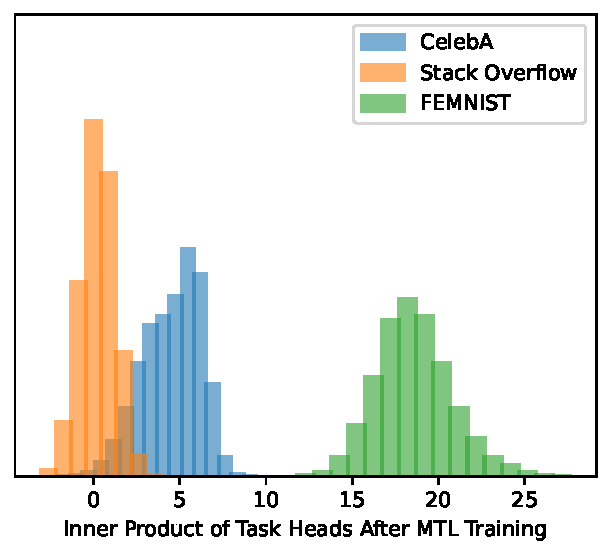
\includegraphics[width=0.4\linewidth]{figs/ablations/task_head_inner_product_hist.pdf}
    \caption{Task-Specific Layer Similarity (Personalization)}
    \label{fig:hist_taskheads}
\end{figure}


% \subsection{Additional Figures} \label{appdx:figs_eval}

% In this section, we provide additional figures for the Evaluation section in the main text.



\subsection{Ablations on Synthetic Data} \label{appdx:synth}

We attempt to understand task-inference leakage by running our attacks on a synthetic dataset. The data generation process for this dataset is identical to the mean estimation example in Section~\ref{sec:mean_est}, but we adapt it for machine learning. To create the synthetic dataset, we start by sampling $2T$ i.i.d. tasks, $\{ \mu_1 \dots \mu_{2T} \}$ from a $d$-dimensional Gaussian distribution. For each of the tasks, $\mu_i$, we sample a dataset of $N$ $d$-dimensional vectors from the corresponding task distribution. To label the data for a learning problem, we first generate a random projection matrix $H \in \mathbb{R}^{k \times d}$, where $d$ is the data dimension and $k$ is the embedding dimension. Then, we randomly sample the "target" task-specific layers $g_1, \dots g_T \in \mathbb{R}^k$ and get the label for each sample, $\vec{x}$, coming from task $\tau \in [T]$ to be the sign of the inner product between $g_\tau$ and the embedding vector $H\vec{x}$ (that is, for any sample $X_{i,j}$, $y_{i,j} = \texttt{sign}(\inn{\: g_i}{ H X_{i,j} \:} )$.  This particular dataset is well suited for MTL as all tasks have unique labeling functions, but a common projection into the embedding space.


In our experiments on synthetic data, we use a simple neural network with 512 hidden units and a linear projection layer into the embedding space to approximate $H$. We vary the embedding dimension, number of samples per task, and number of tasks in the dataset, then measure our coordinate-wise variance attack's AUC over 4 training runs, with 64 trials of each attack on 8 random samples from each task. The results of this experiment are shown in Figure~\ref{fig:synthetic}. We observe that increasing the number of total samples in the dataset, whether by increasing the number of samples per task or the total number of tasks, has a sharp impact on the \textbf{strong} adversary's AUC. As the model has more samples to learn from, the gap between the \textbf{strong} and \textbf{weak} adversary's AUC scores shrinks. We also find that, in this suite of experiments, the embedding dimension has little impact on task-inference AUC.


\begin{figure*}[h]
    \centering
    \begin{subfigure}[b]{0.3\textwidth}
        \centering
        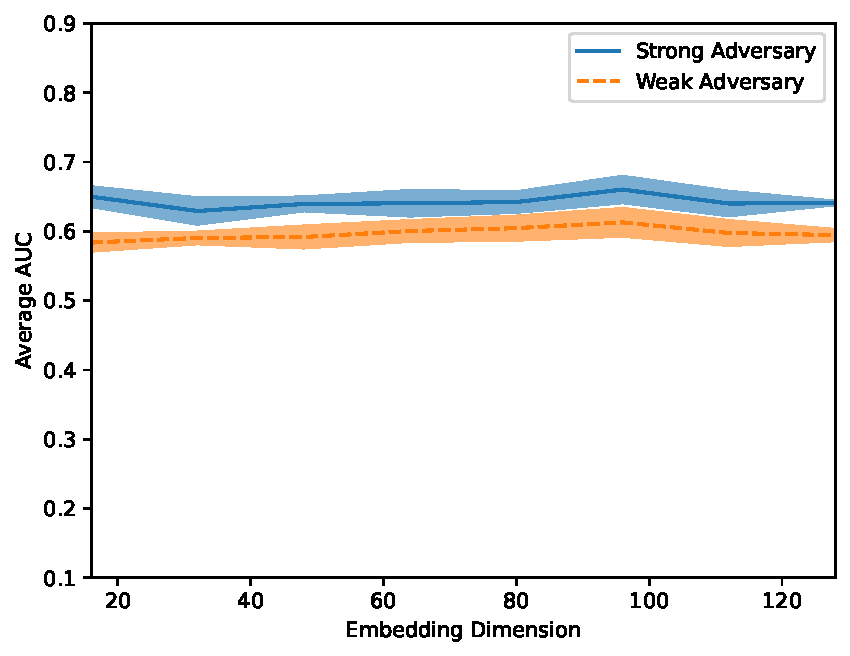
\includegraphics[width=\textwidth]{figs/ablations/hidden_dim_ablation.pdf}
        \caption{Embedding Dimension}
        \label{fig:embedding_dim}
    \end{subfigure}
    \hfill
    \begin{subfigure}[b]{0.3\textwidth}
        \centering
        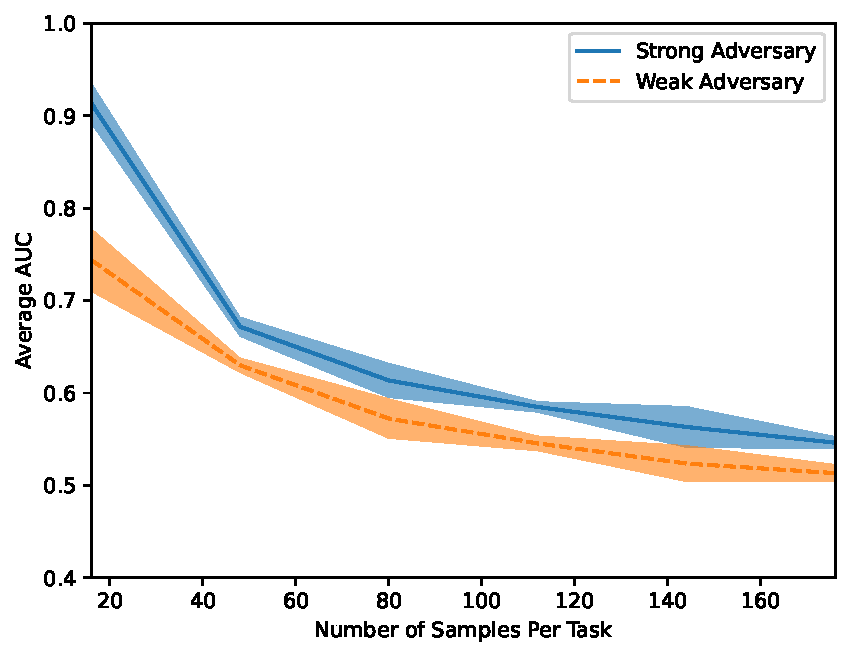
\includegraphics[width=\textwidth]{figs/ablations/num_samples_ablation.pdf}
        \caption{Number of Samples Per Task}
        \label{fig:num_samples}
    \end{subfigure}
    \hfill
    \begin{subfigure}[b]{0.3\textwidth}
        \centering
        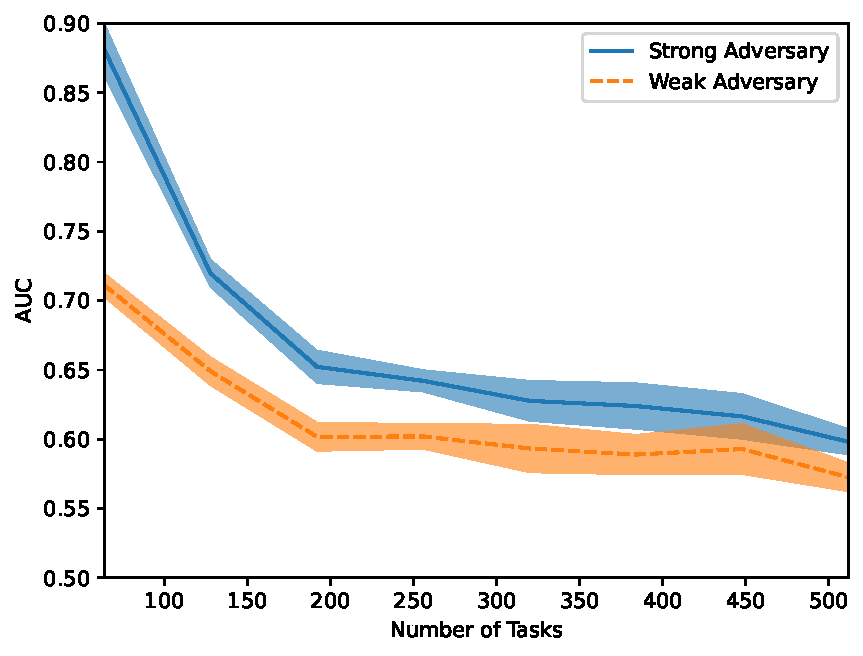
\includegraphics[width=\textwidth]{figs/ablations/num_tasks_ablation.pdf}
        \caption{Number of Tasks}
        \label{fig:num_tasks}
    \end{subfigure}
    \caption{Ablations on Synthetic Data}
    \label{fig:synthetic}
\end{figure*}


% \section{Additional Discussion}

% We provide additional discussion points to supplement Section~\ref{sec:discussion}.

 
